\frame{\frametitle{Low Euclidean distance $\neq$ low distribution similarity}
\begin{itemize}
\item $p_1 \sim \mathcal{N}(\mu_1,\sigma_1)$, $p_2 \sim \mathcal{N}(\mu_2,\sigma_2)$
\end{itemize}
\begin{columns}
\begin{column}{.48\textwidth}
%\color{red}\rule{\linewidth}{4pt}
\begin{block}{\small High Euclidean distance, High Distribution similarity}
{\small
$\mu_1=0,\sigma_1=10K$\\
$\mu_2=10,\sigma_2=10K$
}
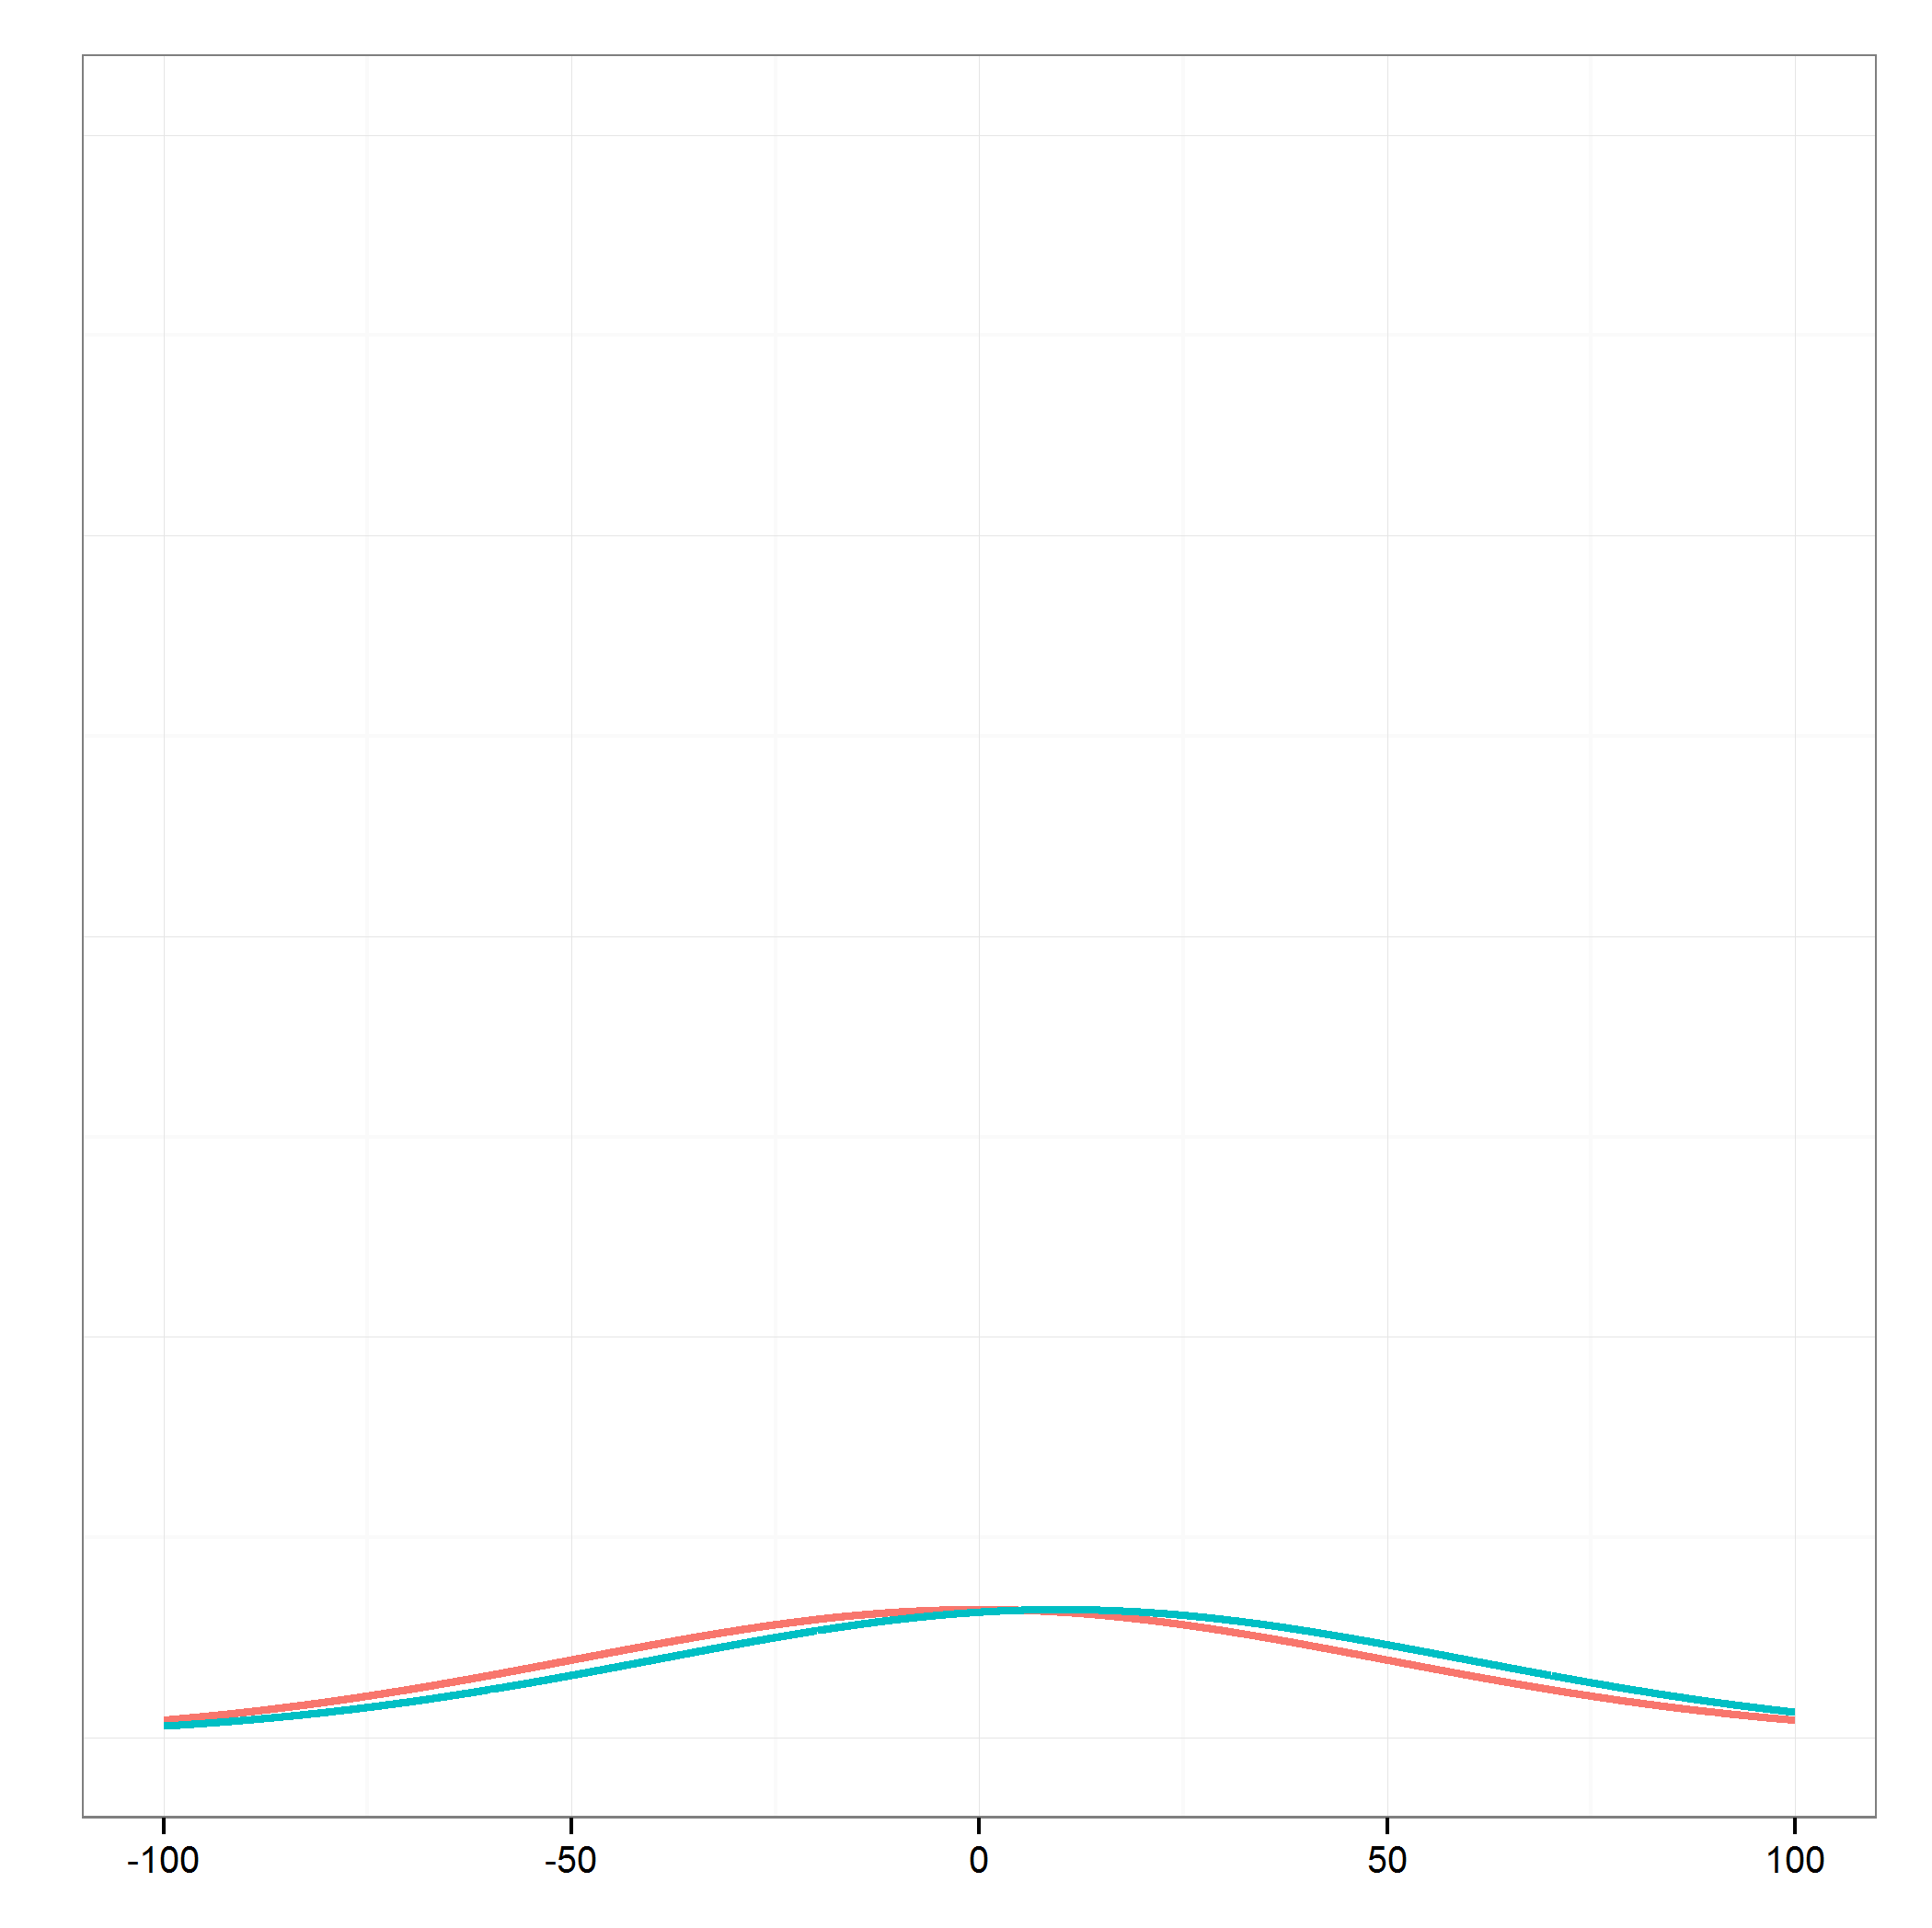
\includegraphics[scale=.3]{figs/first}
\end{block}
\end{column}%
\hfill%
\uncover<2->{
\begin{column}{.48\textwidth}
%\color{blue}\rule{\linewidth}{4pt}
\begin{block}{\small Low Euclidean distance, High Distribution similarity}
{\small
$\mu_1=0,\sigma_1=0.01K$\\
$\mu_2=0.1,\sigma_2=0.01K$
}
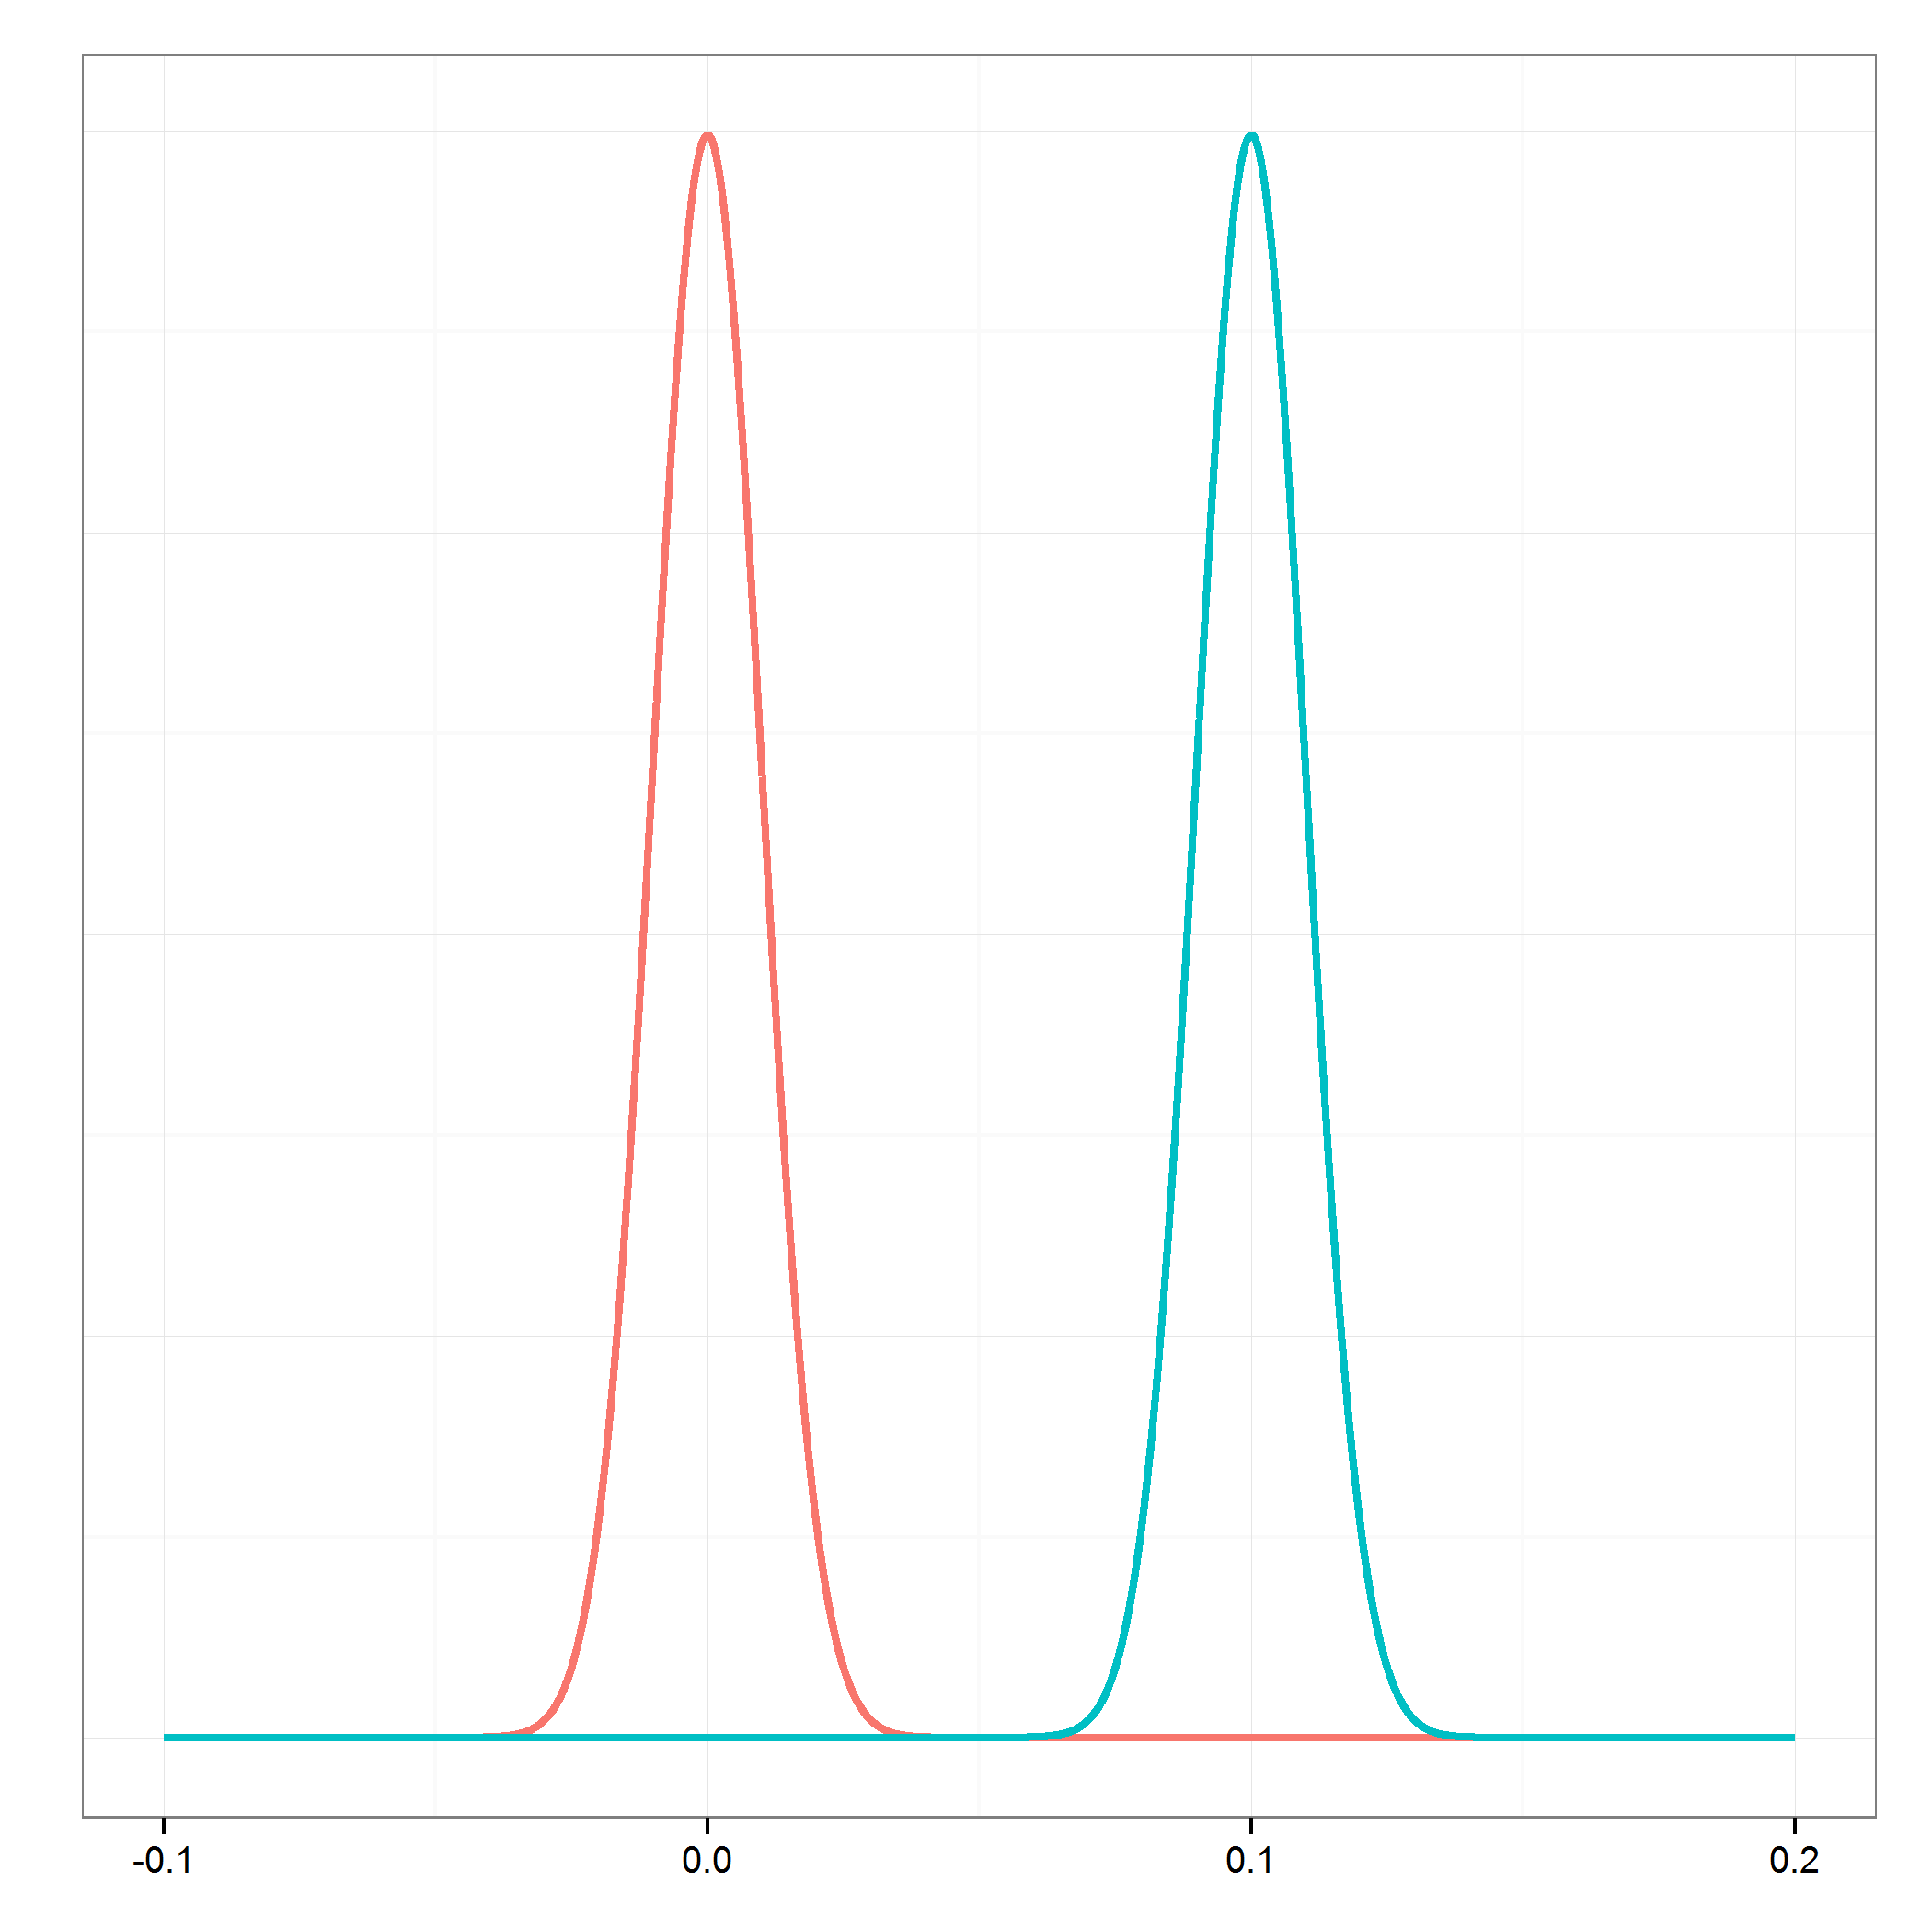
\includegraphics[scale=.3]{figs/second}
\end{block}
\end{column}%
}
\end{columns}
%%%%%%%%%%
}
\frame{\frametitle{Natural Gradient}
 Talk about Natural Gradient
}